%%%%%%%%%%%%%%%%%%%%%%%%%%%%%%%%%%%%%%%%%%%%%%%%%%%%%%%%%%%%%%%%%%%%%%%%%%%%%%%%
%% Title (en): Multiagent Systems and Organizations                           %%
%% Title (cs): Multiagentní systémy a organizace                              %%
%%                                                                            %%
%% Author: Bc. Lukáš Kúdela                                                   %%
%% Supervisor: Prof. RNDr. Petr Štěpánek, DrSc.                               %%
%%                                                                            %%
%% Academic year: 2011/2012                                                   %%
%%%%%%%%%%%%%%%%%%%%%%%%%%%%%%%%%%%%%%%%%%%%%%%%%%%%%%%%%%%%%%%%%%%%%%%%%%%%%%%%

%%%%%%%%%%%%%%%%%%%%%%%%%%%%%%%%%%%%%%%%%%%%%%%%%%%%%%%%%%%%%%%%%%%%%%%%%%%%%%%%
\section{Example 1: Function Invocations}
%%%%%%%%%%%%%%%%%%%%%%%%%%%%%%%%%%%%%%%%%%%%%%%%%%%%%%%%%%%%%%%%%%%%%%%%%%%%%%%%

%%%%%%%%%%%%%%%%%%%%%%%%%%%%%%%%%%%%%%%%%%%%%%%%%%%%%%%%%%%%%%%%%%%%%%%%%%%%%%%%
\subsection*{MAS Specification}

%%%%%%%%%%%%%%%%%%%%%%%%%%%%%%%%%%%%%%%%%%%%%%%%%%%%%%%%%%%%%%%%%%%%%%%%%%%%%%%%
\subsubsection*{Organization Part}

% Function invocation organization
This example demonstrates a simple organization - the \textit{invoke-function} organization (modelled by the \texttt{FunctionInvocation\_Organization} agent class).
% Function invocation organization - purpose
The purpose of the organization is to facilitate function invocation by grouping two agents: the first agent \textit{invokes} a function and the second agent \textit{executes} it.
Thus, the function is invoked in a \textit{remote} way.
The example uses the factorial function, but it should be obvious that any (computable) function can be used instead.

% Function invocation organization - roles
The \textit{Invoke function} organization contains two roles - \textit{Asker} and \textit{Answerer} - and one protocol - \textit{Invoke function}.

% Invoker role
The \textit{Invoker} role (modelled by the \texttt{Invoker\_Role} class) is a single role representing an invoker of a function.
The invoker of a function can request the executer to compute the function.
% Invoker role - competences & responsibilities
The \textit{Invoker} role has one competence - \textit{Invoke function} - and no responsibilities.

% Invoke function competence
The \textit{Invoke function} competence (modelled by the \texttt{InvokeFunction\_Competence} class) is a competence to invoke a function.
% Invoke function competence - argument & result
The competence has one argument - the function argument - and one result - the function value.

% Executer role
The \textit{Executer} role (modelled by the \texttt{Executer\_Role} class) is a single role representing an executer of a function.
The executer function can compute the function upon request.
% Execute role - competences & responsibilities
The \textit{Executer} role has no competences and one responsibility - \textit{Execute function}.

% Execute function responsibility
The \textit{Execute function} responsibility (modelled by the \texttt{ExecuteFunction\_Responsibility} class) is a responsibility to execute a function together with its argument.
% Execute function responsibility - argument & result
The responsibility has one argument - the function argument - and one result - the function value.

%%%%%%%%%%%%%%%%%%%%%%%%%%%%%%%%%%%%%%%%%%%%%%%%%%%%%%%%%%%%%%%%%%%%%%%%%%%%%%%%
\subsubsection*{Protocol Part}

% Invoke function protocol
The \textit{Invoke function} protocol (modelled by the \texttt{InvokeFunctionProtocol}) is a protocol by which the initiator party (modelled by the \texttt{InvokeFunction\_InitiatorParty} class) requests the responder party (modelled by the \texttt{InvokeFunction\_ResponderParty}) to execute a function (the factorial function in this example).

% Request message
The \textit{Request} message (modelled by the \texttt{RequestMessage} class) is a message sent by the \textit{Invoker} to the \textit{Executer} carrying a request to execute the function and its argument.

% Reply message
The \textit{Reply} message (modelled by the \texttt{ReplyMessage} class) is a message sent by the \textit{Executer} to the \textit{Invoker} carrying an information that the function has been executed and its value.

\subsubsection*{Player Part}

% Demo player
The \textit{Demo} player (modelled by the \texttt{Demo\_Player} agent class) is a player capable of computing (ALT: evaluating) the factorial function.

%%%%%%%%%%%%%%%%%%%%%%%%%%%%%%%%%%%%%%%%%%%%%%%%%%%%%%%%%%%%%%%%%%%%%%%%%%%%%%%%
\subsection*{Manifestation}

% Agents - players & organizations
There are two \textit{Demo} players in the running MAS - the \textit{demo1} and \textit{demo2} players (modelled by the \texttt{demo1\_Player} and \texttt{demo2\_Player} agent instances respectively) - and one organization - the \textit{invoke-function} organization (modelled by the \texttt{invokeFunction\_Organization} agent instance).

% Agent intentions
The intention of \textit{demo1} is to invoke a function (factorial in this example) and provide an argument (here 10) and the intention of \textit{demo2} is to execute this function and provide a return value (here 3628800).
Since both players are capable of executing the function (calculating the factorial), the invocation could also happen the other way round.

%%%%%%%%%%%%%%%%%%%%%%%%%%%%%%%%%%%%%%%%%%%%%%%%%%%%%%%%%%%%%%%%%%%%%%%%%%%%%%%%
\subsubsection*{Stage 1: Role Enactment}

% Figure: Stage 1: Role enactment
\begin{figure}[H]
	\centering
	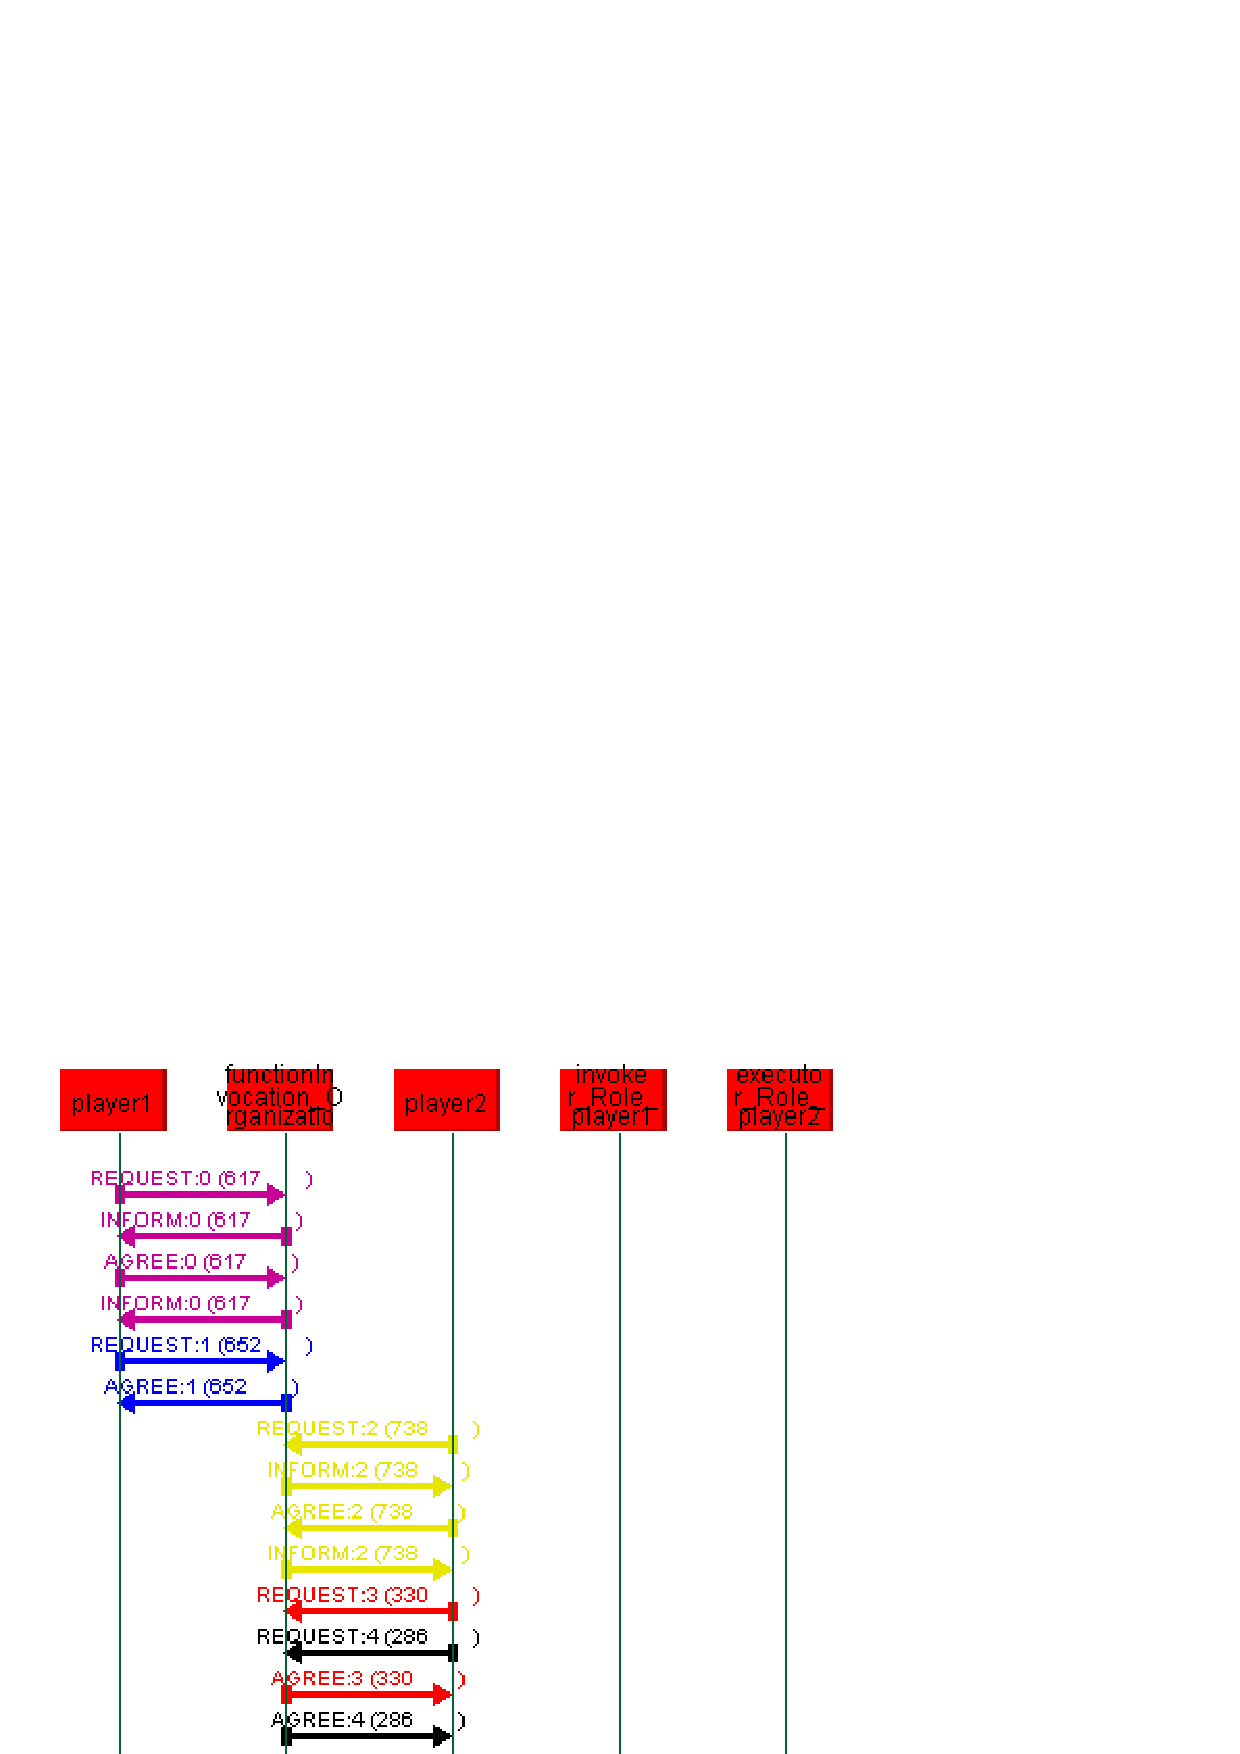
\includegraphics[width=\textwidth]{images/example1-stage1.png}
	\caption{Stage 1: Role enactment}
	\label{figure:example1-stage1}
\end{figure}

% Blue
\textbf{Blue} The blue interaction scenario between the \textit{demo1} player and \textit{invoke function} organization follows the \textit{Enact role} protocol.
\textit{demo1} requests \textit{invoke-function} to enact the \textit{Invoker} role (1\textsuperscript{st} message) and is informed about the role's responsibilities (2\textsuperscript{nd} message) .
Since \textit{Invoker} has no responsibilities, \textit{demo1} agrees that it can indeed enact the role (3\textsuperscript{rd} message).
\textit{invoke-organization} then creates the \textit{invoker-demo1} position (modelled by the \texttt{invoker\_Role\_demo1\_Player} agent instance) and informs \textit{demo1} of its AID (4\textsuperscript{th} message).

% Purple
\textbf{Purple} The purple interaction scenario between the \textit{demo2} player and \textit{invoke function} organization follows the \textit{Enact role} protocol.
\textit{demo2} requests \textit{invoke-function} to enact the \textit{Executer} role (1\textsuperscript{st}) and is informed about the role's responsibilities (2\textsuperscript{nd} message).
Since \textit{demo2} can perform one \textit{Executer}'s responsibility - the \textit{Execute function} responsibility - it agrees that it can indeed enact the role (3\textsuperscript{rd} message).
\textit{invoke-function} then creates the \textit{executer-demo2} position (modelled by the \texttt{executer\_Role\_demo2\_Player} agent instance) and informs \textit{demo2} of its AID (4\textsuperscript{th} message).

%%%%%%%%%%%%%%%%%%%%%%%%%%%%%%%%%%%%%%%%%%%%%%%%%%%%%%%%%%%%%%%%%%%%%%%%%%%%%%%%
\subsubsection*{Stage 2: Role Activation}

% Figure: Stage 2: Role activation
\begin{figure}[H]
	\centering
	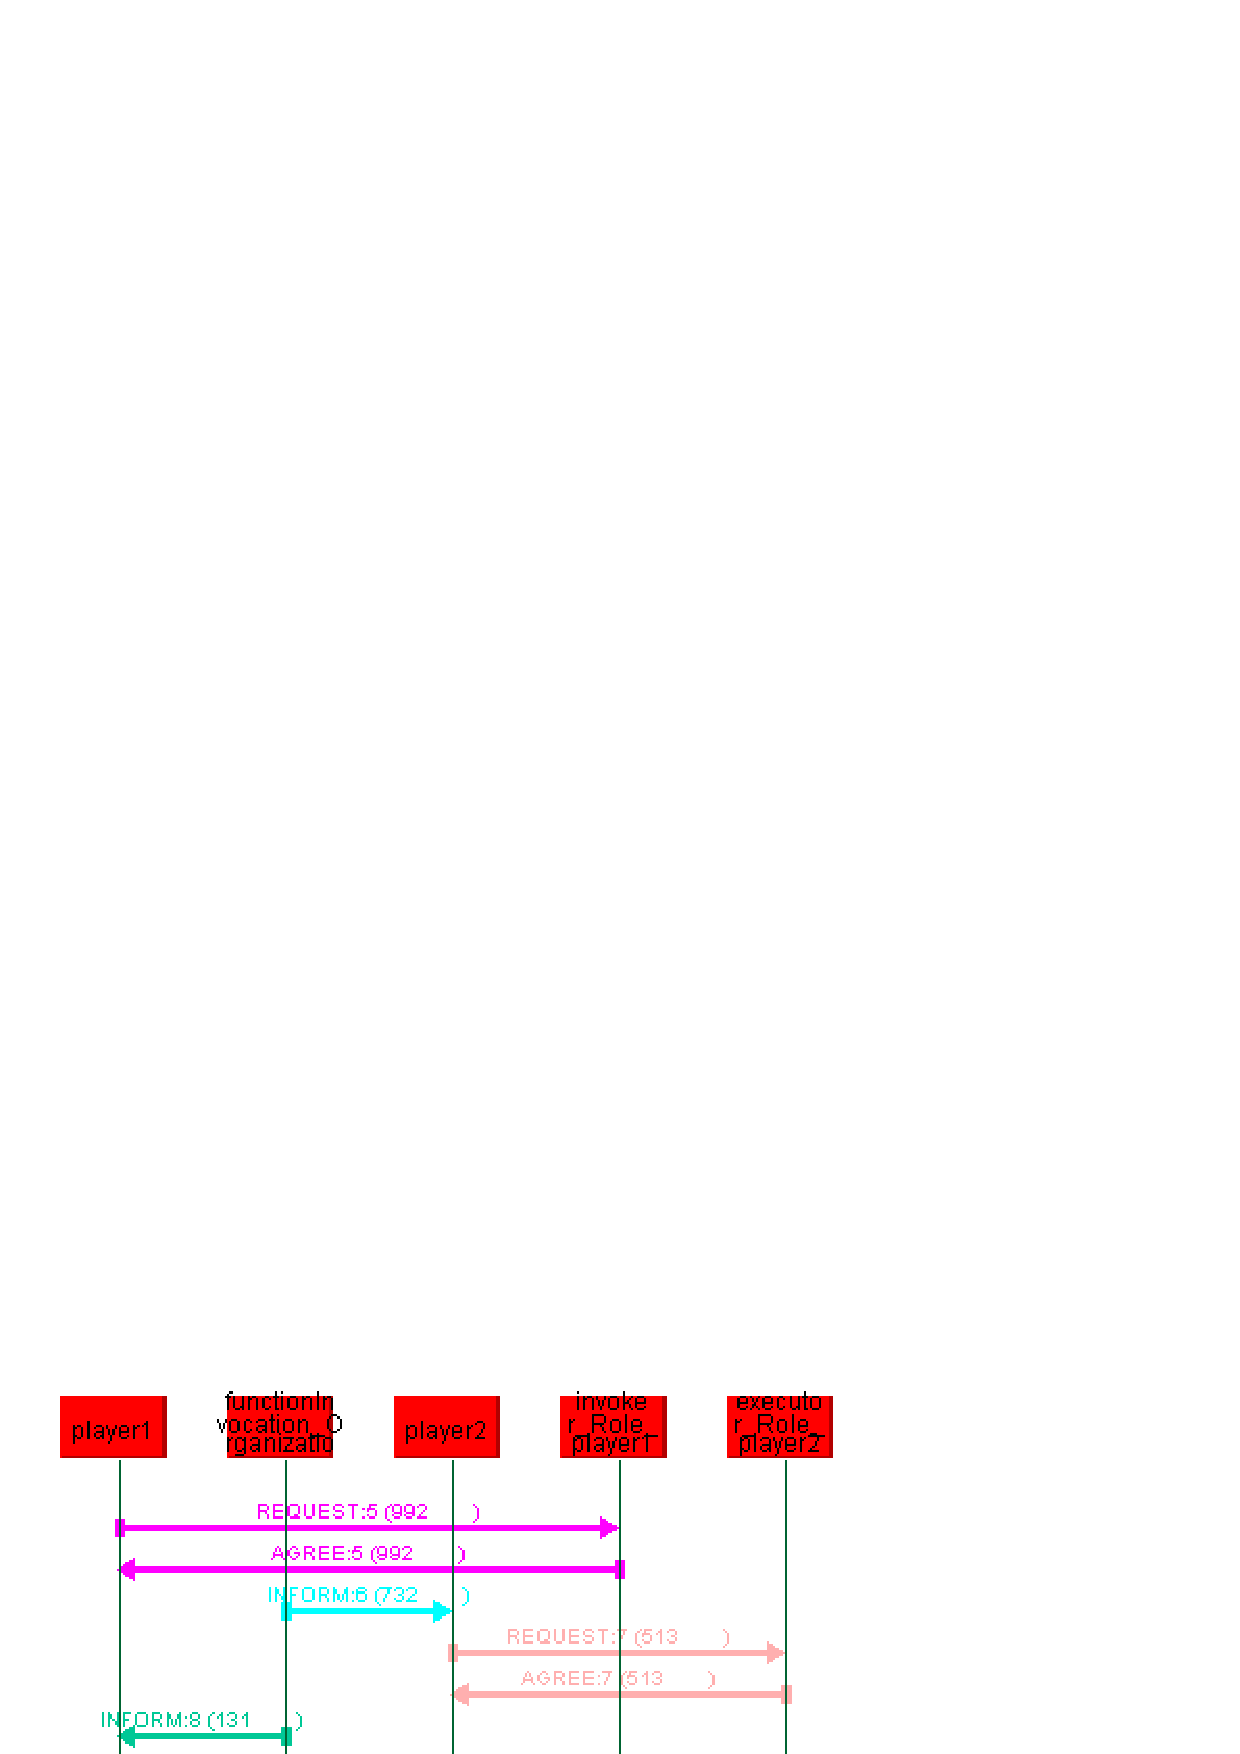
\includegraphics[width=\textwidth]{images/example1-stage2.png}
	\caption{Stage 2: Role activation}
	\label{figure:example1-stage2}
\end{figure}

% Red
\textbf{Red} The red interaction scenario between the \textit{demo1} player and the \textit{invoker-demo1} position follows the \textit{Activate role} protocol.
\textit{demo1} requests \textit{invoker-demo1} to activate the role (1\textsuperscript{st} message) and the position promptly agrees (2\textsuperscript{nd} message).

% Gold
\textbf{Gold} The gold interaction scenario between the \textit{demo2} player and the \textit{executer-demo2} position follows the \textit{Activate role} protocol.
\textit{demo2} requests \textit{executer-demo2} to activate the role (1\textsuperscript{st} message) and the position immediately agrees (2\textsuperscript{nd} message).

%%%%%%%%%%%%%%%%%%%%%%%%%%%%%%%%%%%%%%%%%%%%%%%%%%%%%%%%%%%%%%%%%%%%%%%%%%%%%%%%
\subsubsection*{Stage 3: Competence and Responsibility Invocation}

% Figure: Stage 3: Competence and responsibility invocation
\begin{figure}[H]
	\centering
	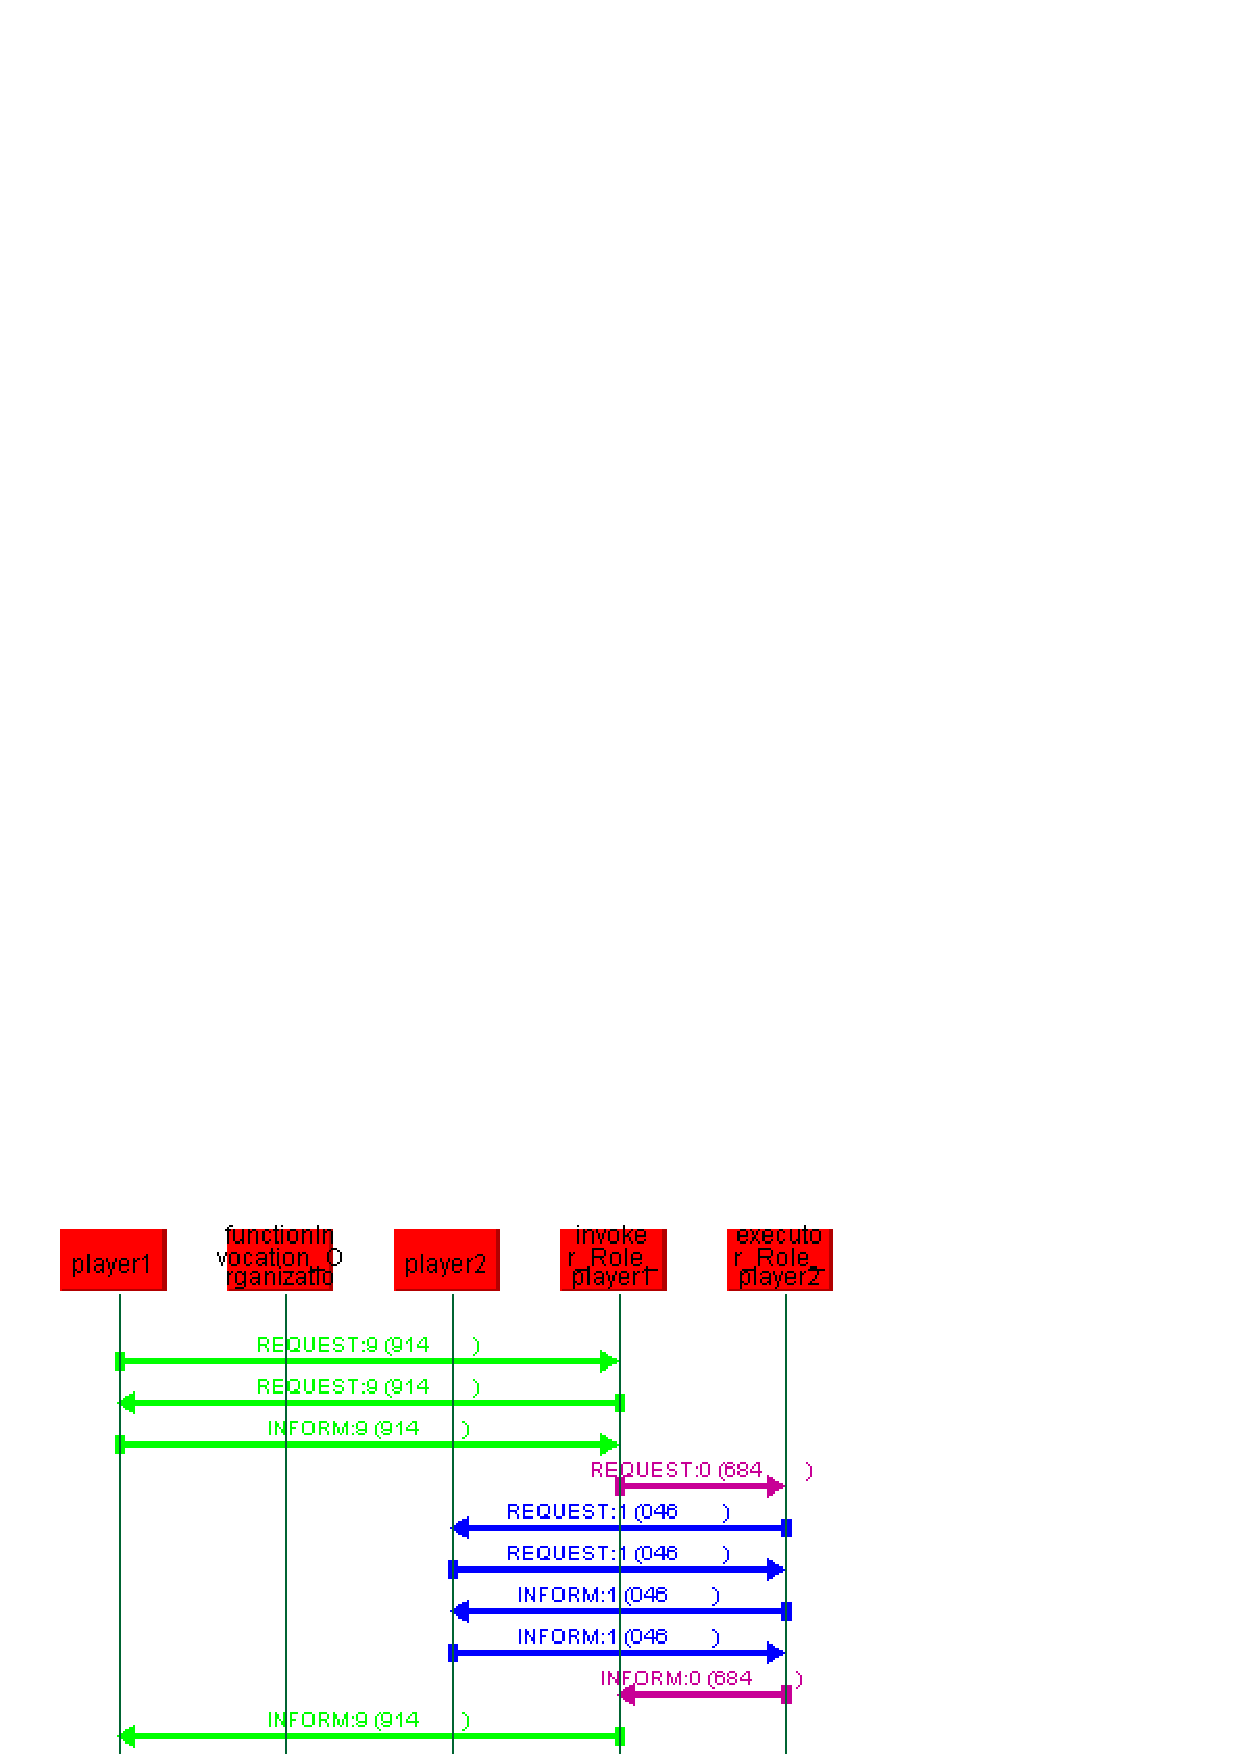
\includegraphics[width=\textwidth]{images/example1-stage3.png}
	\caption{Stage 3: Competence and responsibility invocation}
	\label{figure:example1-stage3}
\end{figure}

% Note - `Invoke competence' protocol vs. 'Invoke function' competence
In the following discussion, is is important to keep in mind that the \textit{Invoke competence} protocol is being used to invoke the \textit{Invoke function} competence.
Understanding the distinction between these two usages of the word `invoke' is a prerequisite to understanding the discussion of Stage 3.

% Black
\textbf{Black} The black interaction scenario between the \textit{demo1} player and the \textit{invoker-demo1} position follows the \textit{Invoke competence} protocol.
\textit{demo1} requests \textit{invoker-demo1} to invoke the \textit{Invoke function} competence (1\textsuperscript{st} message) and is in turn requested to provide the competence argument (2\textsuperscript{nd} message).
\textit{demo1} then promptly informs \textit{invoker-demo1} about the argument (3\textsuperscript{rd} message).
After \textit{invoker-demo1} executes the competence (the magenta interaction scenario), it informs \textit{demo1} about its result (4\textsuperscript{th} message).

% Magenta
\textbf{Magenta} The magenta interaction scenario between the \textit{initiator-demo1} and \textit{executer-demo2} positions follows the \textit{Invoke function} protocol.
\textit{initiator-demo1} requests \textit{executer-demo2} to execute a particular function (factorial) for a particular argument (10, 1\textsuperscript{st} message).
\textit{executer-demo2}, after invoking the \textit{Execute function} responsibility on its player (the cyan interaction scenario), informs \textit{invoker-demo1} about the function return value (3628800, 2\textsuperscript{nd} message).

% Cyan
\textbf{Cyan} The cyan interaction scenario between the \textit{executer-demo2} position and \textit{demo2} player follows the \textit{Invoke responsibility} protocol.
\textit{executer-demo2} requests \textit{demo2} to invoke the \textit{Execute function} responsibility (1\textsuperscript{st} message) and is in turn requested to provide the responsibility argument (2\textsuperscript{nd} message).
\textit{executer-demo2} then immediately informs \textit{demo2} about the argument (3\textsuperscript{rd} message).
After \textit{demo2} executes the responsibility, it informs \textit{executer-demo2} about its result (4\textsuperscript{th} message).

%%%%%%%%%%%%%%%%%%%%%%%%%%%%%%%%%%%%%%%%%%%%%%%%%%%%%%%%%%%%%%%%%%%%%%%%%%%%%%%%
\subsubsection*{Stage 4: Role Deactivation}

% Figure: Stage 4: Role deactivation
\begin{figure}[H]
	\centering
	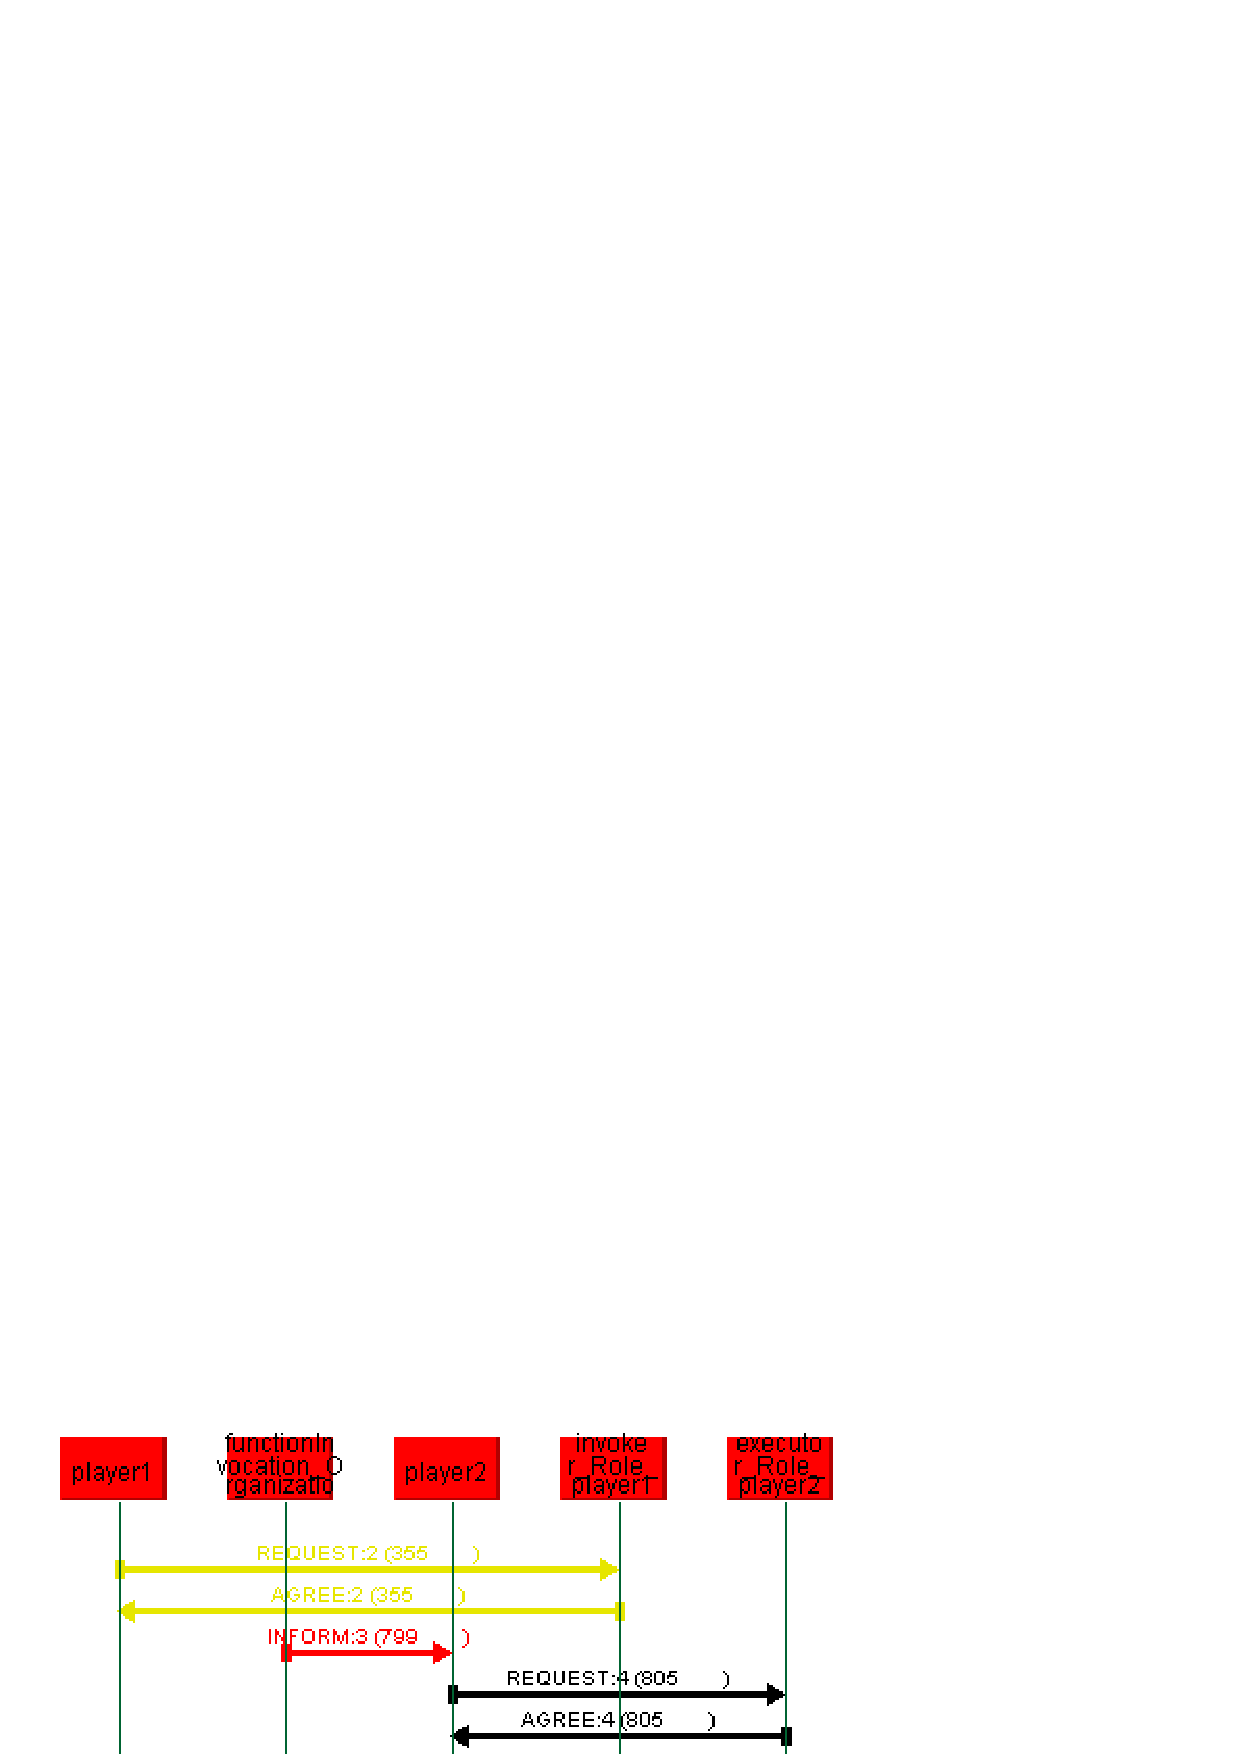
\includegraphics[width=\textwidth]{images/example1-stage4.png}
	\caption{Stage 4: Role deactivation}
	\label{figure:example1-stage4}
\end{figure}

% Pink
\textbf{Pink} The pink interaction scenario between the \textit{demo1} player and the \textit{invoker-demo1} position.
\textit{demo1} requests \textit{invoker-demo1} to deactivate the role (1\textsuperscript{st} message) and the position promptly agrees (2\textsuperscript{nd} message).

% Teal
\textbf{Teal} The teal interaction scenario between the \textit{demo2} player and the \textit{executer-demo2} position.
\textit{demo2} requests \textit{executer-demo2} to deactivate the role (1\textsuperscript{st} message) and the position immediately agrees (2\textsuperscript{nd} message).

%%%%%%%%%%%%%%%%%%%%%%%%%%%%%%%%%%%%%%%%%%%%%%%%%%%%%%%%%%%%%%%%%%%%%%%%%%%%%%%%
\subsubsection*{Stage 5: Role Deactment}

% Figure: Stage 5: Role deactment
\begin{figure}[H]
	\centering
	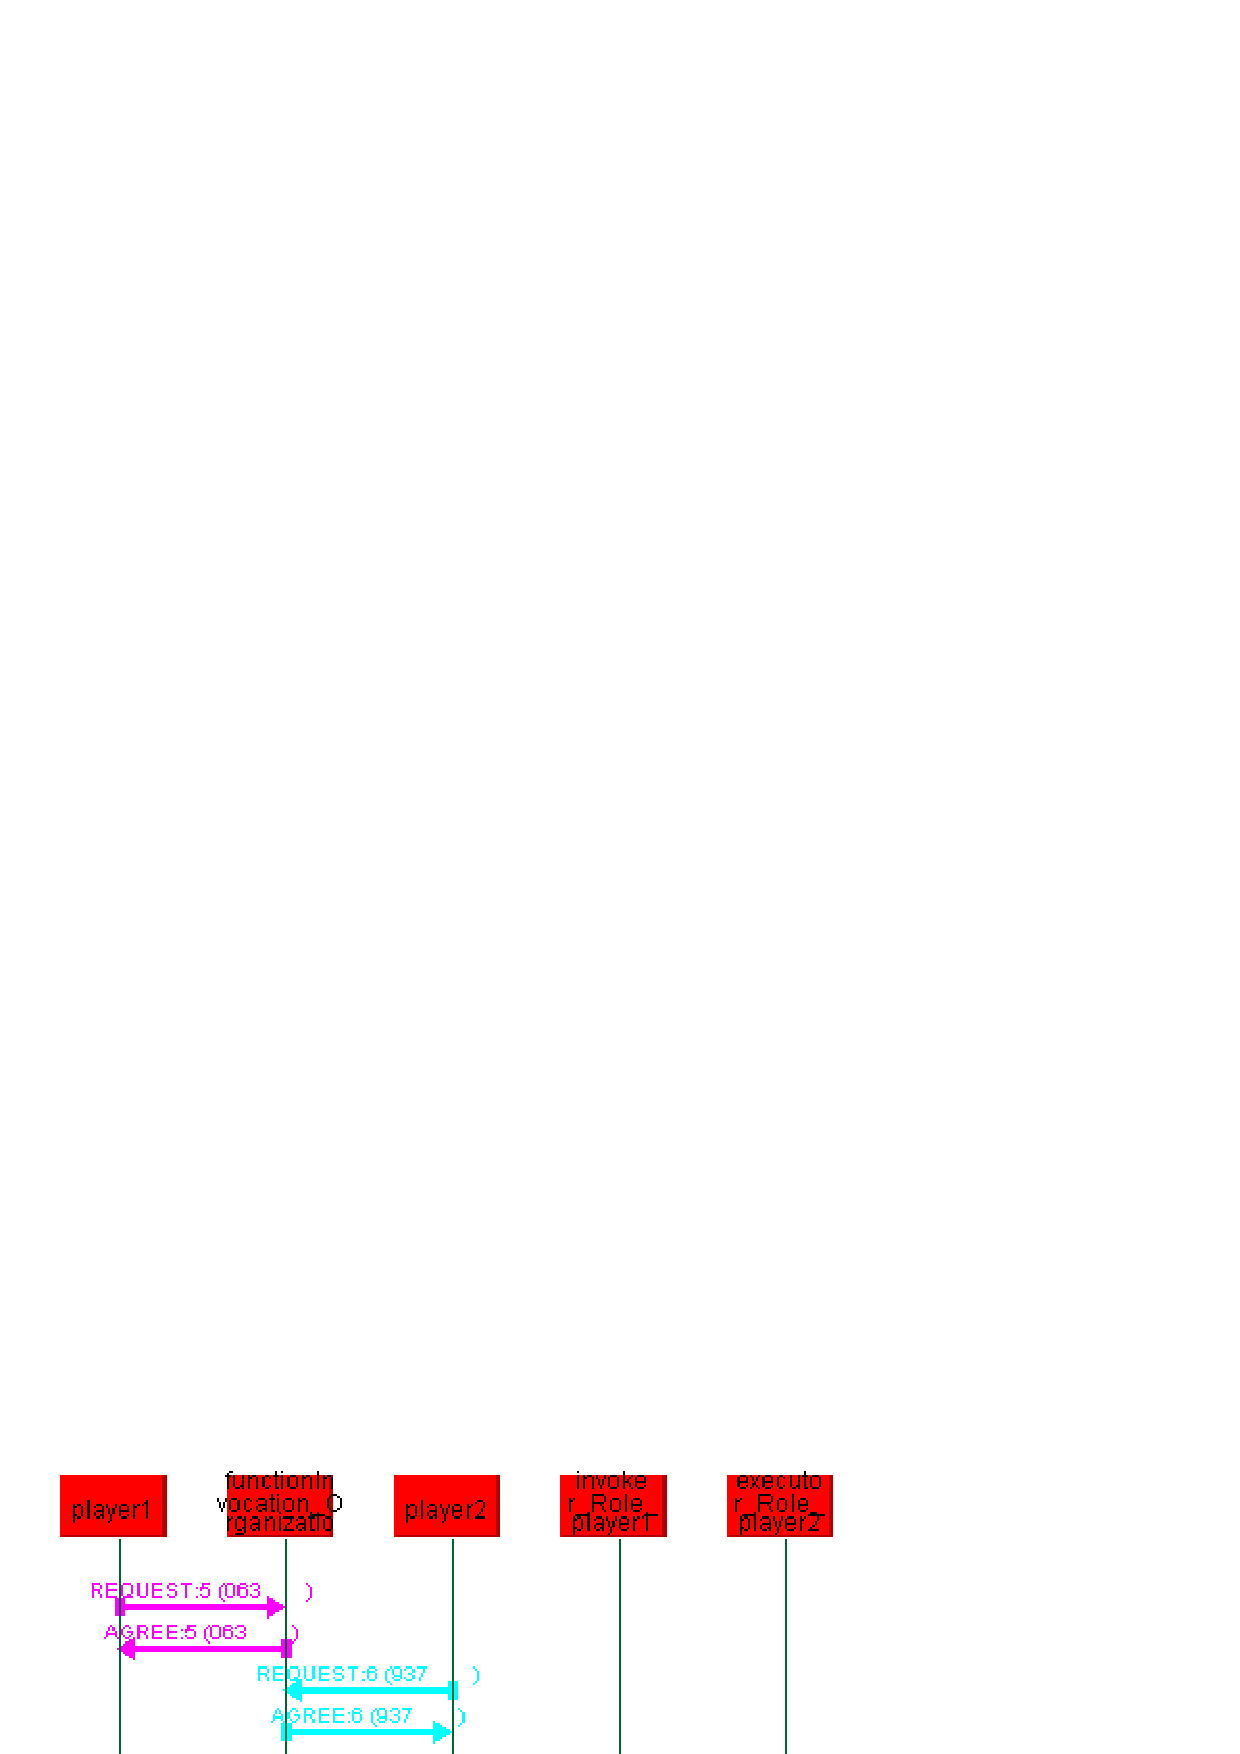
\includegraphics[width=\textwidth]{images/example1-stage5.png}
	\caption{Stage 5: Role deactment}
	\label{figure:example1-stage5}
\end{figure} 

% Green
\textbf{Green} The green interaction scenario between the \textit{demo1} player and the \textit{invoke-function} organization.
\textit{demo1} requests \textit{invoke-function} to deact the \textit{Invoker} role (1\textsuperscript{st} message) and the organization promptly agrees (2\textsuperscript{nd} message).

% Purple
\textbf{Purple} The purple interaction scenario between the \textit{demo2} player and the \textit{invoke-function} organizations.
\textit{demo2} requests \textit{invoke-function} to deact the \textit{Executer} role (1\textsuperscript{st} message) and the organization immediately agrees (2\textsuperscript{nd} message).